\chapter{Cinemática}
A Física como ciência é muito vasta e requer subdivisões de estudo, uma das grandes areas que estuda o movimento em condições específicas é a cinemática. 

A cinemática estuda o movimento dos corpos sem se preocupar com as causas que o produzem, ou seja, a cinemática descreve como os corpos se movem, enquanto a dinâmica estuda por que os corpos se movem.

\section{Conceitos Fundamentais}

Antes de estudarmos o movimento, precisamos entender alguns conceitos básicos, como referencial, ponto material, corpo extenso e trajetória.

\subsection{Referencial e Sistemas de Coordenadas}

O \textbf{referencial} é o corpo ou lugar a partir do qual observamos os fenômenos. Para quantificar essa observação, utilizamos um \textbf{sistema de coordenadas}.

\subsubsection{Sistema de Coordenadas e a Origem}
O sistema de coordenadas \cref{fig:sistemas_coordenadas} permite localizar o móvel no espaço. Todo sistema possui uma \textbf{origem} (Ponto Zero), que é o ponto de referência para a contagem das posições ($s$).

% --- Exemplo de Sistema Unidimensional ---
\begin{figure}[htbp]
    \centering
    % --- Subfigura A: Unidimensional ---
    \begin{subfigure}[b]{0.45\textwidth}
        \centering
        \begin{tikzpicture}[>=stealth, scale=0.8]
            \draw[->, thick] (-2.5,0) -- (2.5,0) node[right] {$s$};
            \foreach \x in {-2,-1,0,1,2}
                \draw (\x, 0.1) -- (\x, -0.1) node[below] {\scriptsize \x};
            \filldraw[azul] (0,0) circle (2pt) node[above=2pt] {\scriptsize $O$};
            \filldraw[vermelho] (1.5,0) circle (2pt);
        \end{tikzpicture}
        \caption{Sistema Unidimensional (Reta)}
        \label{fig:coord_unidim}
    \end{subfigure}
    \hfill % Espaçamento entre as figuras
    % --- Subfigura B: Bidimensional ---
    \begin{subfigure}[b]{0.45\textwidth}
        \centering
        \begin{tikzpicture}[>=stealth, scale=0.6]
            \draw[->, thick] (-1,0) -- (3,0) node[right] {$x$};
            \draw[->, thick] (0,-1) -- (0,3) node[above] {$y$};
            \draw[help lines, dashed] (0,0) grid (2,2);
            \filldraw[azul] (0,0) circle (3pt) node[below left] {\scriptsize $O$};
            \filldraw[vermelho] (2,2) circle (3pt) node[above right] {\scriptsize $P(2,2)$};
        \end{tikzpicture}
        \caption{Sistema Bidimensional (Plano)}
        \label{fig:coord_bidim}
    \end{subfigure}

    \vspace{0.3cm}
    \caption{Representação visual dos sistemas de coordenadas e suas respectivas origens ($O$).}
    \label{fig:sistemas_coordenadas}
\end{figure}

\begin{itemize}
    \item \textbf{Movimento:} Variação da posição ao longo do tempo em relação ao referencial.
    \item \textbf{Repouso:} Posição sem alteração ao longo do tempo de acordo com o referencial adotado.
\end{itemize}

% Exemplo de relatividade do movimento
\begin{figure}[htbp]
    \centering
    \includegraphics[width=0.8\textwidth]{figuras/fig-01.png}
    \caption[Movimento relativo no ônibus]{Ilustração do movimento relativo de uma esfera: Na figura superior, nota-se um passageiro observando o movimento vertical de uma esfera. Na figura inferior, nota-se um observador externo visualizando uma trajetória parabólica da mesma esfera.}
    \label{fig:movimento_relativo}
\end{figure}

Qualquer corpo móvel ou fixo pode ser escolhido como referencial, desde que sua posição seja conhecida. O sistema de coordenadas é definido após estabelecer a métrica que frequentemente assume valores dentro do SI.

\subsubsection{Exemplo Prático}
Considere uma rodovia: o quilômetro zero é a \textbf{origem}. Se um carro está parado no KM 20, ele está em repouso em relação à rodovia, mas em movimento em relação ao Sol \parencite{halliday2012}.

O estado de movimento ou repouso depende do referencial adotado, como ilustrado na \cref{fig:movimento_relativo}.

\subsection{Ponto Material e Corpo Extenso}

A classificação de um móvel depende da escala do fenômeno observado.

\begin{itemize}
    \item \textbf{Ponto Material:} Suas dimensões são desprezíveis em relação ao fenômeno. Ex: Um planeta orbitando o Sol.
    \item \textbf{Corpo Extenso:} Suas dimensões são relevantes e influenciam no estudo. Ex: Um planeta sendo estudado quanto à sua rotação e inclinação do eixo.
\end{itemize}

% Exemplo de ponto material vs corpo extenso
\begin{figure}[htbp]
    \centering
    \includegraphics[width=0.6\textwidth]{figuras/fig-02.png}
    \caption[Movimento relativo no ônibus]{A figura demonstra a diferença entre um ponto material e um corpo extenso. À esquerda, uma pessoa sob uma superfície muito extensa. A direita, uma pessoa em uma superfície pequena, onde suas dimensões são relevantes.}
    \label{fig:corpo_ponto}
\end{figure}

\subsubsection{Critério de Diferenciação}
Para diferenciar, comparamos o tamanho do objeto com o espaço que ele ocupa. Se o tamanho do objeto for muito menor que o espaço, ele pode ser tratado como ponto material; caso contrário, é um corpo extenso \parencite{serway2014}. A \cref{fig:corpo_ponto} ilustra essa distinção.

\subsection{Trajetória}
É o lugar geométrico das posições sucessivas do móvel. Sua forma depende do referencial.

\section{Tipos de Movimento}
\begin{itemize}
    \item \textbf{Progressivo:} $v > 0$ (segue a orientação da via).
    \item \textbf{Retrógrado:} $v < 0$ (contra a orientação da via).
\end{itemize}

\begin{figure}[htbp]
    \centering
    % --- CASO 1: MOVIMENTO PROGRESSIVO ---
    \begin{subfigure}[b]{0.48\textwidth}
        \centering
        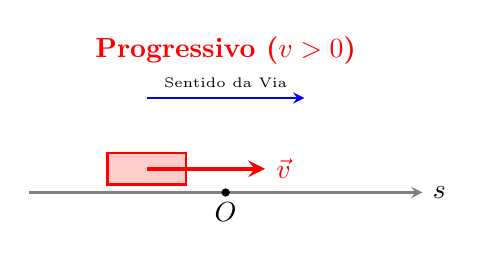
\begin{tikzpicture}[>=stealth]
            % Eixo da trajetória
            \draw[->, thick, gray] (-2.5,0) -- (2.5,0) node[right, black] {$s$};
            \fill (0,0) circle (1.5pt) node[below] {$O$};
            
            % Sentido Positivo da Via
            \draw[->, blue, thick] (-1, 1.2) -- (1, 1.2) node[midway, above, black] {\tiny Sentido da Via};
            
            % O Móvel (Progressivo)
            \draw[fill=red!20, draw=red, thick] (-1.5, 0.1) rectangle (-0.5, 0.5);
            \draw[->, red, ultra thick] (-1, 0.3) -- (0.5, 0.3) node[right] {$\vec{v}$};
            
            \node[red, font=\bfseries] at (0, 1.8) {Progressivo ($v > 0$)};
        \end{tikzpicture}
        \caption{Mesmo sentido da trajetória.}
    \end{subfigure}
    \hfill % Este comando joga o próximo desenho para a outra ponta
    % --- CASO 2: MOVIMENTO RETRÓGRADO ---
    \begin{subfigure}[b]{0.48\textwidth}
        \centering
        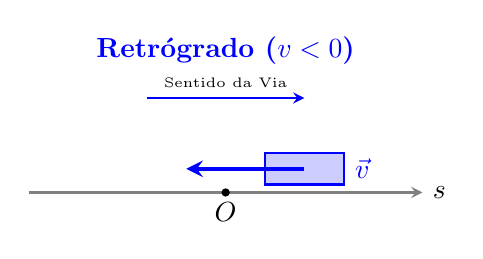
\begin{tikzpicture}[>=stealth]
            % Eixo da trajetória
            \draw[->, thick, gray] (-2.5,0) -- (2.5,0) node[right, black] {$s$};
            \fill (0,0) circle (1.5pt) node[below] {$O$};
            
            % Sentido Positivo da Via
            \draw[->, blue, thick] (-1, 1.2) -- (1, 1.2) node[midway, above, black] {\tiny Sentido da Via};
            
            % O Móvel (Retrógrado)
            \draw[fill=blue!20, draw=blue, thick] (0.5, 0.1) rectangle (1.5, 0.5);
            \draw[<-, blue, ultra thick] (-0.5, 0.3) -- (1, 0.3) node[right, xshift=0.5cm] {$\vec{v}$};
            
            \node[blue, font=\bfseries] at (0, 1.8) {Retrógrado ($v < 0$)};
        \end{tikzpicture}
        \caption{Sentido oposto à trajetória.}
    \end{subfigure}

    \vspace{0.5cm}
    \caption{Classificação do sentido do movimento em relação à orientação da trajetória.}
    \label{fig:progressivo_retrogrado}
\end{figure}

\section{Velocidade}
Mensura a taxa de variação da posição em relação ao tempo. Pode ser classificada em:
\begin{itemize}
    \item \textbf{Velocidade Instantânea:} Grandeza vetorial que indica a velocidade em um instante específico.
    \item \textbf{Velocidade Relativa:} Velocidade de um móvel em relação a outro.
    \item \textbf{Velocidade Escalar Média:} Grandeza escalar que indica a rapidez média de um móvel.
\end{itemize}

No SI a velocidade é medida em metros por segundo (\unit{m/s}). Com isso, podemos entender que um móvel com velocidade de \unit{1}{m/s} percorre \unit{1}{m} a cada segundo. Fator de conversão vide apêndice \ref{apend:fatores_conversao}. 

\subsection{Velocidade Instantânea}
A velocidade instantânea é a taxa de variação da posição num intervalo de tempo próximo a zero. É mensurado com o velocímetro do veículo \ref{fig:velocimetro}. Podemos entender como um limite da velocidade média quando o intervalo de tempo tende a zero. 

% Exemplo de velocidade instantânea
\begin{figure}[htbp]
    \centering
    \includegraphics[width=0.4\textwidth]{figuras/fig-03.png}
    \caption[Velocímetro]{No velocímetro, a velocidade instantânea é indicada pela posição da agulha em um dado instante, refletindo a rapidez do veículo naquele momento específico.}
    \label{fig:velocimetro}
\end{figure}

\section{Velocidade Relativa}

A velocidade relativa é a rapidez com que um corpo se aproxima ou se afasta de outro. Quando analisamos o movimento de dois corpos simultaneamente, muitas vezes é mais simples adotar um dos móveis como referencial "parado" e observar como o outro se move em relação a ele.

\subsection{Movimento na mesma direção e sentido}
Quando dois móveis $A$ e $B$ se deslocam no mesmo sentido, a velocidade relativa ($v_{rel}$) entre eles é dada pela diferença dos módulos das suas velocidades conforme \ref{eq:velocidade_relativa_mesmo_sentido}.

\begin{equation}
    v_{rel} = |v_A - v_B| \label{eq:velocidade_relativa_mesmo_sentido}
\end{equation}

Nesse caso, a velocidade relativa indica o quão rápido um veículo está ganhando distância ou se aproximando para uma ultrapassagem.

\subsection{Movimento na mesma direção e sentidos opostos}
Quando dois móveis caminham um de encontro ao outro (aproximação) ou se afastam em sentidos opostos, a velocidade relativa é dada pela soma dos módulos das suas velocidades.

\begin{equation}
    v_{rel} = |v_A| + |v_B|
\end{equation}



\subsection{Tempo de Encontro e Ultrapassagem}
O conceito de velocidade relativa simplifica drasticamente problemas de encontro. Se dois móveis estão separados por uma distância inicial $\Delta S_{rel}$, o tempo necessário para o encontro ($t_{e}$) ou para a ultrapassagem completa é:

\begin{equation}
    t_{e} = \frac{\Delta S_{rel}}{v_{rel}}
\end{equation}

\subsubsection{Exemplo de Fixação: Ultrapassagem}
Dois carros, $A$ e $B$, movem-se no mesmo sentido em uma estrada com velocidades de \unit{100}{km/h} e \unit{80}{km/h}, respectivamente. Qual a velocidade de $A$ em relação a $B$?

\textit{Resolução:} \\
Como estão no mesmo sentido, subtraímos as velocidades:
\begin{equation*}
    v_{rel} = 100 - 80 = \unit{20}{km/h}
\end{equation*}
Isso significa que, para o motorista do carro $B$, o carro $A$ parece estar se aproximando a apenas \unit{20}{km/h}.

\subsection{Velocidade Escalar Média}
A velocidade escalar média descreve a velocidade em que se deve ter, de maneira fixa, para percorrer uma dada distância naquele tempo. Diferente da velocidade instantânea, essa velocidade descreve todo um trajeto. 
A velocidade média pode ser determinada pela razão entre a distância percorrida ($\Delta S$) com o intervalo de tempo gasto ($\Delta t$), como podemos ver na equação \ref{eq:velocidade_media}.
\begin{equation}
    v_m = \frac{\Delta S}{\Delta t} \label{eq:velocidade_media}
\end{equation}
Com:
\begin{equation*}
    \begin{aligned}
        \Delta S = S - S_0 & \xmapsto{\hspace{1.5cm}} \text{Variação da posição (Deslocamento)} \\
        \Delta t = t - t_0 & \xmapsto{\hspace{1.5cm}} \text{Variação do tempo (Intervalo)} \\
        v_m & \xmapsto{\hspace{1.5cm}} \text{Velocidade Escalar Média}
    \end{aligned}
\end{equation*}

Na figura \ref{fig:veiculo_trajeto}, um veículo percorre um trajeto curvilíneo, saindo da posição $S_0$ no tempo $t_0$ e chegando na posição $S$ no tempo $t$. A velocidade média do veículo é calculada pela razão entre a distância total percorrida e o tempo total gasto. Podemos determinar a velocidade desse veículo aplicando somente a \ref{eq:velocidade_media}.

% Exemplo de velocidade média
\begin{figure}[htbp]
    \centering
    \includegraphics[width=0.4\textwidth]{figuras/fig-04.png}
    \caption[Veículo em trajeto curvilíneo]{Na figura é retratado algumas manobras que um veículo pode realizar. Observe que, o veículo sai da posição $S_0$ no tempo $t_0$ e percorre um trajeto curvilíneo até chegar na posição $S$ no tempo $t$.}
    \label{fig:veiculo_trajeto}
\end{figure}

Podemos compreender a velocidade média como sendo a média ponderada das velocidades instantâneas ao longo do trajeto. 

A ponderação é determinada pelo tempo gasto em cada trecho do percurso. Se um veículo percorre um trajeto com velocidades variáveis, a velocidade média é calculada considerando o tempo gasto em cada trecho e as respectivas velocidades instantâneas. 

Note que, se ter velocidades diferentes em cada trecho, haverá tempos diferentes para percorrer aquela distância, com isso, podemos determinar cada distância percorrida em cada trecho e o tempo gasto, para então calcular a razão com o tempo total e por fim determinar a velocidade média do trajeto. Observe a \ref{eq:vm_ponderada}.
\begin{equation}
    v_m = \frac{\sum_{i=1}^{n} v_i \cdot \Delta t_i}{\sum_{i=1}^{n} \Delta t_i} 
    \implies 
    v_m = \frac{v_1 \Delta t_1 + v_2 \Delta t_2 + v_3 \Delta t_3 + \dots}{ \Delta t_1 + \Delta t_2 + \Delta t_3 + \dots} 
    \label{eq:vm_ponderada}   
\end{equation}

Um caso semelhante é quando um veículo percorre um trajeto variando sua velocidade, muitas vezes em razão das curvas, semáforos ou outros fatores. Vamos ver alguns exemplos. 

\section{Exemplos de Fixação}

\begin{enumerate}[
    label=\textbf{Exemplo \arabic*:}, 
    leftmargin=0pt, 
    itemindent=!, 
    labelsep=0.5em,
    align=left
]

    % --- EXEMPLO 1 ---
    \item \textbf{Cálculo Direto} \\
    \begin{minipage}{\textwidth}
    \noindent Um veículo percorre a distância de \unit{240}{km} entre duas cidades em um intervalo de tempo de \unit{3}{h}. Determine a velocidade média do percurso.
    \end{minipage}

    \textit{Resolução:} \\
    Utilizamos a definição básica de velocidade média:
    \begin{equation}
        v_m = \frac{\Delta S}{\Delta t} \implies v_m = \frac{240}{3} = \unit{80}{km/h} \label{eq:ex_direto_v4}
    \end{equation}

    % --- EXEMPLO 2 ---
    \item \textbf{Posições e Instantes} \\
    \begin{minipage}{\textwidth}
    \noindent Um móvel encontra-se no marco quilométrico $S_0 = \unit{20}{km}$ às 14:00h. Após algum tempo, ele atinge a posição $S = \unit{170}{km}$ às 16:30h. Qual a sua velocidade média?
    \end{minipage}

    \textit{Resolução:} \\
    \noindent Precisamos determinar o deslocamento e o intervalo de tempo:
    \begin{itemize}[leftmargin=1.5em] 
        \item $\Delta S = S - S_0 = 170 - 20 = \unit{150}{km}$
        \item $\Delta t = 16:30 - 14:00 = \unit{2,5}{h}$
    \end{itemize}
    \noindent Aplicando a fórmula da velocidade média:
    \begin{equation}
        v_m = \frac{150}{2,5} = \unit{60}{km/h} \label{eq:ex_posicoes_v4}
    \end{equation}

    % --- EXEMPLO 3 ---
    \item \textbf{Determinando a Distância} \\
    \begin{minipage}{\textwidth}
    \noindent Um avião mantém uma velocidade média de \unit{900}{km/h} durante um voo de \unit{4}{h} \unit{15}{min}. Qual a distância total percorrida pela aeronave?
    \end{minipage}

    \textit{Resolução:} \\
    \noindent Convertendo o tempo para unidade decimal ($\unit{15}{min} = \unit{0,25}{h}$), temos $\Delta t = \unit{4,25}{h}$. Isolando a variação de posição:
    \begin{equation}
        \Delta S = v_m \cdot \Delta t \implies \Delta S = 900 \cdot 4,25 = \unit{3825}{km} \label{eq:ex_distancia_v4}
    \end{equation}

    % --- EXEMPLO 4 ---
    \item \textbf{Previsão de Tempo} \\
    \begin{minipage}{\textwidth}
    \noindent Um ciclista com velocidade constante de \unit{5}{m/s} passa pela posição $S_0 = \unit{100}{m}$ no instante $t=0$. Em quanto tempo ele atingirá a posição $S = \unit{400}{m}$?
    \end{minipage}

    \textit{Resolução:} \\
    \noindent O deslocamento necessário é $\Delta S = S - S_0 = 400 - 100 = \unit{300}{m}$. Isolando o tempo:
    \begin{equation}
        \Delta t = \frac{\Delta S}{v_m} \implies \Delta t = \frac{300}{5} = \unit{60}{s} \text{ (ou 1 minuto)} \label{eq:ex_tempo_v4}
    \end{equation}

    % --- EXEMPLO 5 ---
    \item \textbf{Velocidade Média via Tabela} \\
    \begin{minipage}{\textwidth}
    \noindent Um teste de desempenho monitorou um protótipo em três trechos distintos. Determine a velocidade média total do teste com base nos dados abaixo.
    \end{minipage}

    \begin{table}[H]
        \centering
        \begin{tabular}{ccc}
            \toprule
            Trecho & Velocidade ($v_i$) & Tempo ($\Delta t_i$) \\ \midrule
            1 & \unit{20}{m/s} & \unit{10}{s} \\
            2 & \unit{30}{m/s} & \unit{20}{s} \\
            3 & \unit{15}{m/s} & \unit{10}{s} \\ \bottomrule
        \end{tabular}
    \end{table}

    \textit{Resolução:} \\
    \noindent A velocidade média é a razão entre a distância total ($\sum \Delta S_i$) e o tempo total:
    \begin{equation}
        v_m = \frac{v_1 \Delta t_1 + v_2 \Delta t_2 + v_3 \Delta t_3}{\Delta t_1 + \Delta t_2 + \Delta t_3} = \frac{(20 \cdot 10) + (30 \cdot 20) + (15 \cdot 10)}{10 + 20 + 10} \label{eq:ex_ponderada_v4}
    \end{equation}
    \begin{equation*}
        v_m = \frac{200 + 600 + 150}{40} = \frac{950}{40} = \unit{23,75}{m/s}
    \end{equation*}

\end{enumerate}

\section{Questões:}

\begin{enumerate}
    \item No estudo da cinemática, dizemos que o repouso e o movimento são conceitos relativos. Explique o que isso significa e qual a importância do \textbf{referencial} nessa definição.
    
    \item Imagine um passageiro dentro de um trem que se desloca com velocidade constante em uma linha férrea retilínea. O passageiro solta uma moeda. 
    \begin{enumerate}[label=\alph*)]
        \item Qual a trajetória da moeda para o passageiro?
        \item Qual a trajetória da moeda para um observador parado na plataforma da estação?
    \end{enumerate}

    \item Diferencie \textbf{ponto material} de \textbf{corpo extenso}. É possível que um mesmo objeto (como um transatlântico) seja considerado ponto material em uma situação e corpo extenso em outra? Justifique.

    \item Um motorista observa o velocímetro de seu carro e nota que a agulha marca exatamente \unit{100}{km/h}. Esse valor refere-se à velocidade escalar média ou à velocidade escalar instantânea? Justifique sua resposta.

    \item O que caracteriza um movimento como \textbf{retrógrado}? Nesse caso, o valor da velocidade escalar média será positivo ou negativo?

    \item Um atleta completa uma volta em uma pista circular de \unit{400}{m}. 
    \begin{enumerate}[label=\alph*)]
        \item Qual foi o deslocamento ($\Delta S$) do atleta ao final da volta?
        \item A distância percorrida por ele é igual ao seu deslocamento? Explique.
    \end{enumerate}

    \item No Sistema Internacional de Unidades (SI), qual é a unidade padrão para a velocidade? Por que no cotidiano é mais comum utilizarmos o \unit{}{km/h} em vez da unidade do SI?

    \item Considere uma rodovia onde a orientação da trajetória cresce de Sul para Norte. Um carro que viaja de uma cidade ao Norte para uma cidade ao Sul está realizando um movimento progressivo ou retrógrado? Por quê?
\end{enumerate}

\section{Exercícios}

\begin{enumerate}
    \item Um automóvel percorre uma distância de \unit{450}{km} em \unit{5}{h}. Calcule a velocidade escalar média do veículo nesse trajeto em \unit{}{km/h}.
    
    \item Um móvel parte da posição $S_0 = \unit{15}{m}$ e, após \unit{10}{s}, encontra-se na posição $S = \unit{85}{m}$. Determine a sua velocidade média no Sistema Internacional (SI).
    
    \item Uma aeronave comercial voa com velocidade média de \unit{800}{km/h}. Quanto tempo ela levará para completar um percurso de \unit{2400}{km} entre dois aeroportos?
    
    \item Um corredor mantém uma velocidade constante de \unit{4}{m/s}. Qual a posição $S$ do atleta após \unit{1}{min} de corrida, sabendo que ele partiu da origem das posições ($S_0 = 0$)?
    
    \item Um trem de \unit{200}{m} de comprimento atravessa um túnel de \unit{300}{m} com velocidade constante de \unit{20}{m/s}. Quanto tempo o trem leva para atravessar completamente o túnel?
    
    \item Converta as seguintes velocidades de \unit{}{km/h} para \unit{}{m/s} ou vice-versa:
    \begin{enumerate}[label=\alph*)]
        \item \unit{72}{km/h}
        \item \unit{10}{m/s}
        \item \unit{108}{km/h}
        \item \unit{30}{m/s}
    \end{enumerate}

    \item Um motorista viaja de uma cidade A até uma cidade B. Ele percorre os primeiros \unit{120}{km} com velocidade de \unit{60}{km/h} e os \unit{120}{km} seguintes com velocidade de \unit{40}{km/h}. Qual a velocidade média para o trajeto total de \unit{240}{km}?
    
    \item Um protótipo de testes realiza um circuito dividido em três etapas, conforme a tabela abaixo:

    \begin{table}[H]
        \centering
        \begin{tabular}{ccc}
            \toprule
            Etapa & Velocidade ($v_i$) & Tempo ($\Delta t_i$) \\ \midrule
            A & \unit{10}{m/s} & \unit{20}{s} \\
            B & \unit{25}{m/s} & \unit{10}{s} \\
            C & \unit{15}{m/s} & \unit{10}{s} \\ \bottomrule
        \end{tabular}
    \end{table}
    
    Com base nos dados, determine a velocidade média total do protótipo ao longo de todo o circuito.

    \item Dois automóveis, $A$ e $B$, movem-se em uma estrada retilínea com velocidades constantes $v_A = \unit{80}{km/h}$ e $v_B = \unit{60}{km/h}$. Determine a velocidade relativa de $A$ em relação a $B$ nas seguintes situações:
    \begin{enumerate}[label=\alph*)]
        \item Quando os dois movem-se no mesmo sentido.
        \item Quando os dois movem-se em sentidos opostos.
    \end{enumerate}

    \item Dois trens de carga deslocam-se em trilhos paralelos no mesmo sentido. O trem $A$ tem comprimento de \unit{150}{m} e velocidade de \unit{15}{m/s}, enquanto o trem $B$ tem \unit{100}{m} e velocidade de \unit{10}{m/s}. Quanto tempo o trem $A$ leva para ultrapassar completamente o trem $B$?

    \item Dois ciclistas partem simultaneamente de dois pontos de uma ciclovia, distantes \unit{500}{m} um do outro. O ciclista $A$ parte da posição $S_{0A} = \unit{0}{m}$ com velocidade constante de \unit{8}{m/s}, e o ciclista $B$ parte de $S_{0B} = \unit{500}{m}$ com velocidade constante de \unit{12}{m/s}, em sentidos opostos (indo um de encontro ao outro).
    \begin{enumerate}[label=\alph*)]
        \item Qual o módulo da velocidade relativa de aproximação entre os ciclistas?
        \item Após quanto tempo ocorrerá o encontro?
        \item Em que posição $S$ da ciclovia eles se encontrarão?
    \end{enumerate}

    \item Um barco tenta atravessar um rio perpendicularmente à margem com uma velocidade própria de \unit{4}{m/s}. Sabendo que a velocidade da correnteza do rio é de \unit{3}{m/s}, determine o módulo da velocidade resultante do barco em relação à margem (referencial fixo na terra).

\end{enumerate}

\section{Problemas}

\begin{enumerate}
    \item \textbf{(Encontro de Móveis)} Dois ciclistas, $A$ e $B$, partem simultaneamente das posições $S_{0A} = \unit{0}{m}$ e $S_{0B} = \unit{2000}{m}$ de uma ciclovia retilínea. O ciclista $A$ move-se com velocidade constante $v_A = \unit{15}{m/s}$ e o ciclista $B$ com $v_B = \unit{10}{m/s}$, ambos em sentidos opostos (um de encontro ao outro).
    \begin{enumerate}[label=\alph*)]
        \item Determine o módulo da velocidade relativa de aproximação entre os ciclistas.
        \item Calcule o instante $t$ em que eles se encontram.
        \item Determine a posição $S$ do encontro em relação à origem das posições.
    \end{enumerate}

    \item \textbf{(Ultrapassagem de Corpo Extenso)} Um trem de carga possui comprimento total de \unit{250}{m} e viaja com velocidade constante de \unit{54}{km/h}. Ele deve atravessar completamente uma ponte ferroviária de \unit{150}{m} de extensão.
    \begin{enumerate}[label=\alph*)]
        \item Converta a velocidade do trem para o Sistema Internacional (\unit{}{m/s}).
        \item Qual a distância total que o trem deve percorrer para atravessar completamente a ponte?
        \item Quanto tempo, em segundos, o trem leva para concluir a travessia?
    \end{enumerate}

    \item \textbf{(Velocidade Média em Trechos)} Um motorista deseja realizar uma viagem de \unit{300}{km} com uma velocidade média total de \unit{100}{km/h}. Nos primeiros \unit{150}{km}, devido ao tráfego intenso, ele conseguiu manter uma velocidade média de apenas \unit{75}{km/h}.
    \begin{enumerate}[label=\alph*)]
        \item Qual foi o tempo gasto para percorrer a primeira metade da viagem?
        \item Qual deve ser a velocidade média na segunda metade do percurso para que o motorista consiga atingir seu objetivo inicial de \unit{100}{km/h} para a viagem toda?
    \end{enumerate}
\end{enumerate}